\chapter{Measuring distance to wall}
\label{chap:wall_dist}

\section{IR sensor}
The IR sensors that is used is the SHARP 2d120x which is a nonlinear devise. The IR sensor works by sending a infrared beam out, the beam then returns  back to the device after hitting a surface or a obstacle, the angle that the beam returns with determines the distance. 
  \begin{figure}[!h!]
	\centering
	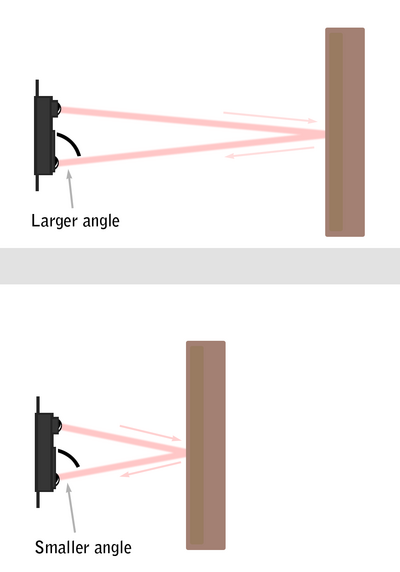
\includegraphics[width=0.15\textwidth]{irsensor.png}
	\caption{Distance IR sensor}
	\label{fig:3}
\end{figure}

\section{Converting using an ADC}
The IR sensor returns a voltage value that is converted in to a unsigned binary one byte number in the MCU's ADC (Analog to Digital Converter) but because of the nonlinearity in the device a equation is made by plotting measurements from 1cm to 50cm. A best fitting trend line it made and from that a equation is used with the output from the ADC to give the distance in cm.
  \begin{figure}[!h]
	\centering
	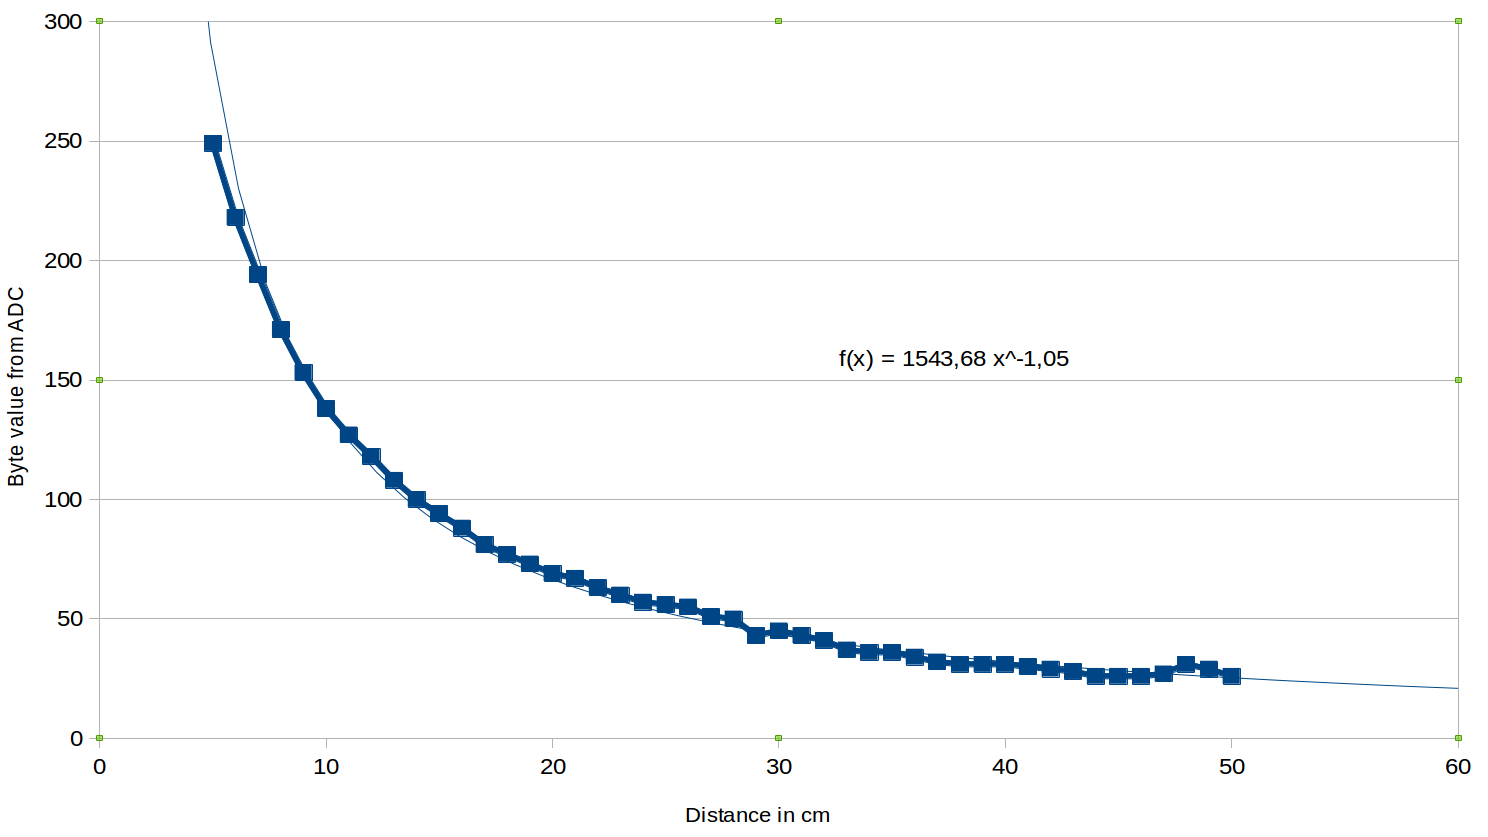
\includegraphics[width=0.8\textwidth]{adcgraf.png}
	\caption{Distance IR sensor}
	\label{fig:3}
\end{figure}

The equations is then fund to be:

\begin{equation}
f(x) = 1543.68
  x^{-1.05}
\end{equation}



\section{Practical use of IR sensors }
%How we inplemented it to solving obstacles around the track.
%Why do we use two of them?
On the track is a variety of different obstacles and some of them require informations about distance. To solve these tasks the robot needs a devise to measuring distance. 

The two obstacle where the IR sensors is used:
\begin{itemize}
	\begin{item}
		\textbf{ Obstacle 1}\\ Go to the wall stop 20cm from the wall turn and return to the line.
	\end{item}
	
	\begin{item}
		\textbf{ Obstacle 2}\\Go around the corner with a distance of 20cm to the wall and stop at the cross marked on the floor. 
	\end{item}
\end{itemize}

There is a total of three IR sensor on board the robot, one at the front just underneath the PS3 camera and two on the left side of the robot. The front sensor it used to solve both obstacle 1 and 2 and outputs a distance to any thing in front of the robot. The two side mounted sensor it used to solve obstacle 2 where the robot shout ''stick'' to the wall by a given distance. 
The implementation of the two side mounted IR sensor it done by using a predefined set point that represent the desired distance to the wall. The two distances from the IR sensors (dist1, dist2) and the set point are then used to calculate the error that corrects the speed to the two DC-motors. All the information from the three IR sensors are send via the I2C bus to the raspberry pi to be processed and is then included in a state machines.
% ---------------------------------------- det sidste er måske ikke så relevant her ???
% indsæt algorithme her !!!
  \begin{figure}[!h!]
	\centering
	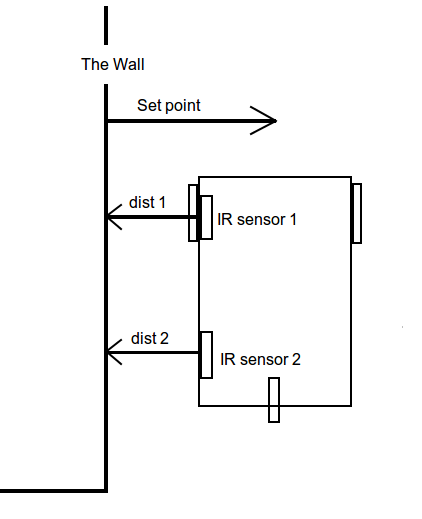
\includegraphics[width=0.5\textwidth]{wall_robot.png}
	\caption{Stick to the wall}
	\label{fig:3}
\end{figure}



      





